%%%%%%%%%%%%%%%%%%%%%%%%%%%%%%%%%%%%%%%%%%%%%%%%%%%%%%%%%%%%%%%%%%%%%%%%%%%%%%%%%%%%%%%%%%%%%%%%%%%
%\documentclass[11pt,mathserif]{beamer}
%\documentclass[serif,mathserif,professionalfont]{beamer}
%\usetheme[block=fill,progressbar=frametitle]{metropolis}
\documentclass[serif,mathserif,professionalfont]{beamer}
\usetheme{Madrid}
\usecolortheme{whale}
\usepackage[T1]{fontenc}
\usepackage[utf8]{inputenc}
\usepackage[spanish]{babel}
\usepackage{amsmath}
\usepackage{amsfonts}
\usepackage{amssymb}
\usepackage{graphicx}

% numeros con punto decimal, no coma
\decimalpoint

% para la bibliografia
\usepackage[style=verbose,backend=bibtex]{biblatex}
\bibstyle{abbrv}

% codigo de R
\usepackage{listings}
\usepackage{color}

% para las tablitas
\usepackage{booktabs}

% para tablas de colores
\usepackage{xcolor,colortbl}
\usepackage{multirow}

%\usefonttheme[onlymath]{mathserif}
%\usepackage{mathpazo} 
%\usepackage[scaled ]{helvet}  
%\usepackage{concmath}

\usepackage{pxfonts}
\usepackage{eulervm}


% intento de incluir animaciones
\usepackage{movie15}

%%%%%%%%%%%%%%%%%%%%%%%%%%%%%%%%%%%%%%%%%%%%%%%%%%%%%%%%%%%%%%%%%%%%%%%%%%%%%%%%%%%%%%%%%%%%%%%%%%%

% parametros de sweave
%\SweaveOpts{concordance=TRUE}

%%%%%%%%%%%%%%%%%%%%%%%%%%%%%%%%%%%%%%%%%%%%%%%%%%%%%%%%%%%%%%%%%%%%%%%%%%%%%%%%%%%%%%%%%%%%%%%%%%%

% retoques graficos para el codigo en R
\newsavebox{\caja}

%%%%%%%%%%%%%%%%%%%%%%%%%%%%%%%%%%%%%%%%%%%%%%%%%%%%%%%%%%%%%%%%%%%%%%%%%%%%%%%%%%%%%%%%%%%%%%%%%%%

% comandos para tablas
\newcommand{\bordes}[1]{\renewcommand{\arraystretch}{#1}}
\definecolor{gray}{rgb}{0.5,0.5,0.5}
\definecolor{gris}{gray}{0.925}
\definecolor{gris2}{gray}{0.8}

%%%%%%%%%%%%%%%%%%%%%%%%%%%%%%%%%%%%%%%%%%%%%%%%%%%%%%%%%%%%%%%%%%%%%%%%%%%%%%%%%%%%%%%%%%%%%%%%%%%

% bibliografia
\addbibresource{referencias_estacionariedad.bib}
\addbibresource{referencias_fisiologia.bib}
\addbibresource{referencias_otros.bib}
\addbibresource{referencias_mixto.bib}

\renewcommand{\footnotesize}{\tiny}

%%%%%%%%%%%%%%%%%%%%%%%%%%%%%%%%%%%%%%%%%%%%%%%%%%%%%%%%%%%%%%%%%%%%%%%%%%%%%%%%%%%%%%%%%%%%%%%%%%%

\newtheorem{definicion}{Definición}
\newtheorem{teorema}{Teorema}
\newtheorem{proposicion}{Proposición}
\newtheorem{demostracion}{Demostración}

\newcommand{\R}{\mathbb{R}}
\newcommand{\C}{\mathbb{C}}
\newcommand{\N}{\mathbb{N}}
\newcommand{\Z}{\mathbb{Z}}
\newcommand{\intR}{\int_{-\infty}^{\infty}}
\newcommand{\intZ}{\int_{-\infty}^{0}}
\newcommand{\intPI}{\int_{-\pi}^{\pi}}
\newcommand{\simint}[1]{\int_{- #1 }^{ #1 }}
\newcommand{\prima}{^{\prime}}

\newcommand{\ddd}{$\delta$}
\newcommand{\dirac}{$\delta$  de Dirac}

\newcommand{\aste}[1]{\widehat{ #1 }^{\star}}
\newcommand{\est}[1]{\widehat{ #1 }}

\newcommand{\COS}[1]{\mathrm{cos}\left( #1 \right)}
\newcommand{\SEN}[1]{\mathrm{sen}\left( #1 \right)}

\newcommand{\E}[1]{\mathrm{E}\left[ #1 \right]}
\newcommand{\Var}[1]{\mathrm{Var}\left( #1 \right)}
\newcommand{\Cov}[1]{\mathrm{Cov}\left( #1 \right)}
\newcommand{\abso}[1]{\left| #1 \right|}

\newcommand{\xt}{$\{X(t)\}_{t\in \boldsymbol{T}}$ }
\newcommand{\xtd}{$\{x_t\}_{t=0,\dots,N}$ }
\newcommand{\orden}{\mathcal{O}}

\newcommand{\talque}{\mathrel{}\middle|\mathrel{}}

\newcommand{\lp}{\ell^{p}}
\newcommand{\llp}{L^{p}[I]}
\newcommand{\ldos}{\ell^{2}}
\newcommand{\lldos}{L^{2}[I]}

\newcommand{\sip}{\ding{51}}
\newcommand{\nop}{\ding{55}}

\newcommand{\pz}{\phantom{.0}}
\newcommand{\ppu}{\phantom{1}}
\newcommand{\phm}{\phantom{-}}

\newcommand{\hz}{\si{\hertz}}
\newcommand{\mv}{\si{\micro\volt}}

%%%%%%%%%%%%%%%%%%%%%%%%%%%%%%%%%%%%%%%%%%%%%%%%%%%%%%%%%%%%%%%%%%%%%%%%%%%%%%%%%%%%%%%%%%%%%%%%%%%

% titulo y fecha
\author[Enciso Alva, J. C.]{Julio Cesar Enciso Alva}
\title[Estacionariedad en PSG de Adultos Mayores]{Estacionariedad débil en registros polisomnográficos
de adultos mayores}
%\setbeamercovered{transparent} 
\setbeamertemplate{navigation symbols}{} 
%\logo{} 
\institute[]{Instituto de Ciencias Básicas e Ingeniería\\ 
Universidad Autónoma del Estado de Hidalgo} 
%\date{\emph{Neuroscience Short Course}\\
%Noviembre de 2017} 
\date{6 de Diciembre de 2017}
%\subject{} 

%%%%%%%%%%%%%%%%%%%%%%%%%%%%%%%%%%%%%%%%%%%%%%%%%%%%%%%%%%%%%%%%%%%%%%%%%%%%%%%%%%%%%%%%%%%%%%%%%%%

\begin{document}

%\metroset{background=dark}

\begin{frame}
\titlepage
\end{frame}

%\begin{frame}
%\tableofcontents
%\end{frame}

%\metroset{background=light}

%%%%%%%%%%%%%%%%%%%%%%%%%%%%%%%%%%%%%%%%%%%%%%%%%

%\section{Introducción}

\section{Introducci\'on}

%%%%%%%%%%%%%%%%%%%%%%%%%%%%%%%%%%%%%%%%%%%%%%%%%%%%%%%%%%%%%%%%%%%%%%%%%%%%%%%%%%%%%%%%%%%%%%%%%%%

\subsection{Antecedentes}

\begin{frame}\frametitle{Antecedentes}
\begin{itemize}
\item Censo Población y Vivienda 2010: 10 millones de AM\footcite{Censo10}
\begin{itemize}
\item Encuesta Intercensal 2015: 12 y medio millones de AM\footcite{Intercensal15}
\end{itemize}

\item Posible relaci\'on: DC en AM y trastornos del sue\~no\footcite{Miyata13}

\item Posible relación: PDC en AM y atrofia del hipocampo + cabmios en el EEG\footcite{Brayet16}

\item Epidemiolog\'ia del DC en Hidalgo: eficiencia del sue\~no \footcite{VazquezTagle16}

%\item DFA en registros de PSG \footcite{Valeria}: exponente de Hurst diferente en sujetos con y 
%sin DC 

%\item Se buscan marcadores cl\'inicos para el diagn\'ostico de DC
\end{itemize}
\end{frame}

%%%%%%%%%%%%%%%%%%%%%%%%%%%%%%%%%%%%%%%%%%%%%%%%%%%%%%%%%%%%%%%%%%%%%%%%%%%%%%%%%%%%%%%%%%%%%%%%%%%
%%%%%%%%%%%%%%%%%%%%%%%%%%%%%%%%%%%%%%%%%%%%%%%%%%%%%%%%%%%%%%%%%%%%%%%%%%%%%%%%%%%%%%%%%%%%%%%%%%%

%\subsection{Objetivos}

%\begin{frame}\frametitle{Pregunta de investigaci\'on}
%%\textbf{
%¿Las características estadísticas\footnote{Particularmente la estacionariedad débil} 
%de los registros PSG puede ser usadas como marcadores diagn\'ostico 
%para deterioro cognitivo en adultos mayores?
%%}
%\end{frame}

%%%%%%%%%%%%%%%%%%%%%%%%%%%%%%%%%%%%%%%%%%%%%%%%%%%%%%%%%%%%%%%%%%%%%%%%%%%%%%%%%%%%%%%%%%%%%%%%%%%
%%%%%%%%%%%%%%%%%%%%%%%%%%%%%%%%%%%%%%%%%%%%%%%%%%%%%%%%%%%%%%%%%%%%%%%%%%%%%%%%%%%%%%%%%%%%%%%%%%%
%%%%%%%%%%%%%%%%%%%%%%%%%%%%%%%%%%%%%%%%%%%%%%%%%%%%%%%%%%%%%%%%%%%%%%%%%%%%%%%%%%%%%%%%%%%%%%%%%%%

\section{Conceptos}

\subsection{Fisilogía}

\begin{frame}\frametitle{Deterioro Cognitivo}
\begin{definicion}[Demencia]
Síndrome que consiste en el desarrollo de déficit cognoscitivos 
suficientemente graves como para interferir significativamente en las actividades laborales y 
sociales, respecto al nivel de actividad previo. \\
Los sujetos con demencia tienen una baja capacidad para aprender información nueva y suelen olvidar 
lo aprendido anteriormente, siendo éste el síntoma más prominente\footcite{DCM5}.
\end{definicion}
\end{frame}

\begin{frame}\frametitle{Pruebas neuropsicológicas}
\begin{itemize}
\item Estado cognoscitivo general
\begin{itemize}
\item {Evaluación Neuropsicológica (\textbf{Neuropsi})} %\cite{Solis03}
\item {Mini Mental State Examination (\textbf{MMSE})} %\cite{Velasco15}
\end{itemize}
\item Detectar pseudodemencia depresiva y ansiedad
\begin{itemize}
\item {Escala breve para la detección de ansiedad del anciano (\textbf{SATS})} %\cite{Vargas11}
\item {Escala de Depresión Geriátrica (\textbf{GDS})} %\cite{Yesavage82,Greenberg12}
\end{itemize}
\item Detectar cambios en la vida cotidiana
\begin{itemize}
\item {Escala sobre las actividades cotidianas de la vida diaria (\textbf{KATZ})} %\footcite{Roumec14}
\end{itemize}
\end{itemize}
\end{frame}

\begin{frame}
\frametitle{Conceptos}
\begin{description}
\item[Sue\~no] Proceso vital c\'iclico complejo y activo
\item[S. MOR] Fase m\'as profunda, alta actividad cerebral, se producen enso\~naciones, 
\textit{sue\~no parad\'ojico}
\begin{itemize}
\item Movimientos oculares r\'apidos
\item Aton\'ia muscular
\item Actividad cerebral desincronizada
\end{itemize}
\end{description}
\end{frame}

\begin{frame}\frametitle{Sustrato fisiológico}
\begin{figure}
\centering
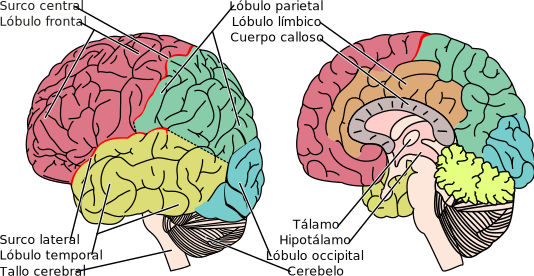
\includegraphics[width=0.9\linewidth]{./img_diagramas/cerebro_zonas_limpio.pdf} 
%\caption{División de la corteza cerebral en lóbulos}
\end{figure}
\end{frame}

\begin{frame}\frametitle{Polisomnograma: EEG}
\begin{figure}
\centering
\includegraphics[width=0.9\linewidth]{./img_diagramas/cabeza_proporcionada_color_v2.pdf} 
%\caption{Sistema de referencia 10--20}
\end{figure}
\end{frame}

\begin{frame}\frametitle{Polisomnograma: EOG + EMG}
\begin{figure}
\centering
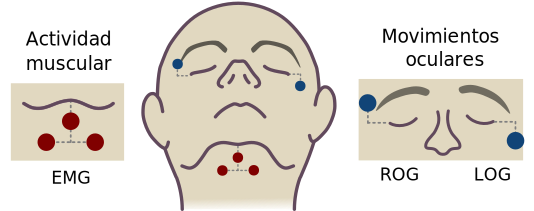
\includegraphics[width=0.9\linewidth]{./img_diagramas/emg_eog_v3.pdf} 
%\caption{Sistema de referencia 10--20}
\end{figure}
\end{frame}

\begin{frame}\frametitle{Registro de PSG}
\begin{figure}
\centering
\includegraphics[width=0.9\linewidth]{./img_ejemplos/MJNN_epoca_stam.pdf}
%\caption{PSG: 19 electrodos EEG, 4 electrodos EOG (horizontal y vertical), 2 electrodos EMG en 
%m\'usculos submentonianos}
\end{figure}
\end{frame}

%%%%%%%%%%%%%%%%%%%%%%%%%%%%%%%%%%%%%%%%%%%%%%%%%%%%%%%%%%%%%%%%%%%%%%%%%%%%%%%%%%%%%%%%%%%%%%%%%%%

\subsection{Matem\'aticas}

%%%%%%%%%%%%%%%%%%%%%%%%%%%%%%%%%%%%%%%%%%%%%%%%%
%%%%%%%%%%%%%%%%%%%%%%%%%%%%%%%%%%%%%%%%%%%%%%%%%

\begin{frame}\frametitle{Conceptos}

\begin{definicion}[Funci\'on de densidad espectral, FDE]
Sea $\{X(t)\}$ un proceso estoc\'astico a tiempo continuo, d\'ebilmente estacionario
\begin{equation*}
h(\omega) = \lim_{T\rightarrow \infty} \E{ \frac{ \left| G_T(\omega) \right|^{2}}{2 T} }
\end{equation*}
Donde $\displaystyle G_T (\omega) = \frac{1}{\sqrt{2 \pi}} \int_{-T}^{T} X(t) e^{-i \omega t} dt$
\end{definicion}
\end{frame}

\begin{frame}\frametitle{Conceptos}
\begin{definicion}[Estacionariedad d\'ebil]
Un proceso estoc\'astico es d\'ebilmente estacionario si y s\'olo si para cualesquiera tiempos 
admisibles $t$, $s$ se tiene que
\begin{itemize}
\item $\E{X(t)} = \mu_X$
\item $\Var{X(t)} = \sigma^{2}_X$
\item $\Cov{X(t),X(s)} = \rho_X (s-t)$
\end{itemize}
Con $\mu_X$, $\sigma^{2}_X$ constantes, $\rho_X(\tau)$ \'unicamente depende de $\tau$
\end{definicion}
\end{frame}

%%%%%%%%%%%%%%%%%%%%%%%%%%%%%%%%%%%%%%%%%%%%%%%%%
%%%%%%%%%%%%%%%%%%%%%%%%%%%%%%%%%%%%%%%%%%%%%%%%%

\begin{frame}\frametitle{FDE vs Autocorrelación}
\begin{teorema}[Wiener-Khinchin]
Una condici\'on suficiente y necesaria para que $\rho$ sea funci\'on de autocorrelaci\'on para 
alg\'un proceso a tiempo continuo d\'ebilmente estacionario y estoc\'asticamente continuo, 
$\{X(t)\}$,  es que exista una funci\'on $F$ tal que
\begin{itemize}
\item Es mon\'otonamente creciente
\item $F(-\infty) = 0$
\item $F(+\infty) = 1$
\item Para todo $\tau \in \R$ se cumple que
\begin{equation*}
\rho(\tau) = \intR e^{i \omega \tau} dF(\omega)
\end{equation*}
\end{itemize}
\end{teorema}
\end{frame}

%%%%%%%%%%%%%%%%%%%%%%%%%%%%%%%%%%%%%%%%%%%%%%%%%
%%%%%%%%%%%%%%%%%%%%%%%%%%%%%%%%%%%%%%%%%%%%%%%%%

\begin{frame}\frametitle{Representaci\'on de Wold-Cram\'er}
\begin{teorema}
Sea $\{X(t)\}$ un proceso a tiempo continuo, d\'ebilmente estacionario, estoc\'asticamente 
continuo, de media 0 y varianza finita. Entonces, existe un proceso ortogonal $\{Z(\omega)\}$ tal 
que
\begin{equation*}
X(t) = \intR e^{i t \omega} dZ(\omega)
\end{equation*}
El proceso $\{Z(t)\}$ cumple para todo $\omega$
\begin{itemize}
\item $\E{dZ(\omega)} = 0$
\item $\E{\abso{dZ(\omega)}^{2}} = dH(\omega)$
\item $\Cov{dZ(\omega),dZ(\lambda)} = 0 \Leftrightarrow \omega \neq \lambda$
\end{itemize}
Con $H$ la SDF integrada de $\{X(t)\}$
\end{teorema}
\end{frame}

\begin{frame}\frametitle{Espectro evolutivo}
Se consideran procesos no-estacionarios, estoc\'asticamente continuos, de media cero y varianza 
finita, y que admitan una representaci\'on de la forma
\begin{equation*}
X(t) = \intPI A(t,\omega) e^{i t \omega} dZ(\omega)
\end{equation*}
tal que 
\begin{itemize}
\item $\Cov{dZ(\omega),dZ(\lambda)} = 0 \Leftrightarrow \omega \neq \lambda$
\item $\E{\abso{dZ(\omega)}^{2}} = \mu(\omega)$
\end{itemize}

El \textbf{espectro evolutivo} fue definido por Priestley \footcite{Priestley65} como
\begin{equation*}
f(t,\omega) = \abso{A(t,\omega)}^{2}
\end{equation*}
\end{frame}

%%%%%%%%%%%%%%%%%%%%%%%%%%%%%%%%%%%%%%%%%%%%%%%%%
%%%%%%%%%%%%%%%%%%%%%%%%%%%%%%%%%%%%%%%%%%%%%%%%%

\begin{frame}%\frametitle{Estimador de doble ventana}
\begin{definicion}[Estimador de doble ventana]
Se define a $\est{f}$, estimador para la $f$, como
\begin{equation*}
\widehat{f}(t,\omega) = \int_{t-T}^{t} w_{T'}(u) \lvert U(t-u,\omega) \lvert^{2} du
\end{equation*}

\begin{itemize}
\item $U(t,\omega) = \int_{t-T}^{t} g(u) X({t-u}) e^{i \omega (t-u)} du$

\item $2\pi \int_{-\infty}^{\infty} \lvert g(u) \lvert^{2} du = 
\int_{-\infty}^{\infty} \lvert \Gamma(\omega) \lvert^{2} d\omega = 1$
\item $w_{\tau}(t) \geq 0$ para cualesquiera $t$, $\tau$
\item $w_{\tau}(t) \rightarrow 0$ cuando $\lvert t \lvert \rightarrow \infty$, para todo $\tau$
\item $\int_{-\infty}^{\infty} w_{\tau}(t) dt = 1$ para todo $\tau$
\item $ \int_{-\infty}^{\infty} \left( w_{\tau}(t) \right)^{2} dt < \infty$ para todo $\tau$
\item $\exists C$ tal que  
$ \lim_{\tau\rightarrow\infty} \tau \int_{-\infty}^{t} \abso{ W_{\tau}(\lambda) }^{2} d\lambda = C$
\end{itemize}
\end{definicion}
\end{frame}

%%%%%%%%%%%%%%%%%%%%%%%%%%%%%%%%%%%%%%%%%%%%%%%%%
%%%%%%%%%%%%%%%%%%%%%%%%%%%%%%%%%%%%%%%%%%%%%%%%%

\begin{frame}
\begin{proposicion}
El estimador $ Y(t,\omega) = \log{\left( \est{f}(t,\omega)\right)}$ satisface que
\begin{itemize}
\item $\displaystyle 
\E{ Y(t,\omega) } \approx \log \left( f(t,\omega) \right)$
\item $\displaystyle 
\Var{ Y(T,\omega) } 
\approx \frac{C}{\tau} \intR \abso{\Gamma (\theta)}^{4} d\theta $
\end{itemize}
\end{proposicion}

M\'as a\'un, puede escribirse
\begin{equation*}
Y(t,\omega) = \log \left( f(t,\omega) \right) + \varepsilon(t,\omega)
\end{equation*}
donde las variables $\varepsilon(t,\omega)$ satisfacen que
\begin{itemize}
\item $\displaystyle \E{\varepsilon(t,\omega)} = 0$
\item $\displaystyle \Var{\varepsilon(t,\omega)}
\approx \frac{C}{\tau} \intR \abso{\Gamma (\theta)}^{4} d\theta$
\end{itemize}
\end{frame}

%%%%%%%%%%%%%%%%%%%%%%%%%%%%%%%%%%%%%%%%%%%%%%%%%
%%%%%%%%%%%%%%%%%%%%%%%%%%%%%%%%%%%%%%%%%%%%%%%%%

%%%%%%%%%%%%%%%%%%%%%%%%%%%%%%%%%%%%%%%%%%%%%%%%%%%%%%%%%%%%%%%%%%%%%%%%%%%%%%%%%%%%%%%%%%%%%%%%%%%
%%%%%%%%%%%%%%%%%%%%%%%%%%%%%%%%%%%%%%%%%%%%%%%%%%%%%%%%%%%%%%%%%%%%%%%%%%%%%%%%%%%%%%%%%%%%%%%%%%%

\section{Metodolog\'ia}

%%%%%%%%%%%%%%%%%%%%%%%%%%%%%%%%%%%%%%%%%%%%%%%%%%%%%%%%%%%%%%%%%%%%%%%%%%%%%%%%%%%%%%%%%%%%%%%%%%%

\subsection{Participantes}

%%%%%%%%%%%%%%%%%%%%%%%%%%%%%%%%%%%%%%%%%%%%%%%%%
%%%%%%%%%%%%%%%%%%%%%%%%%%%%%%%%%%%%%%%%%%%%%%%%%

\begin{frame}\frametitle{Sujetos}
Criterios de inclusi\'on:
\begin{itemize}
\item Firma del consentimiento informado
\item Edad entre 60 y 85 a\~nos
\item Diestros (mano derecha dominante)
\item Sin ansiedad, depresi\'on o s\'indromes focales
\item No usar medicamentos o sustancias para dormir
\item Voluntario para el registro de PSG
\end{itemize}

\textbf{10 participantes: 5 CTL, 5 PDC}
\end{frame}

%%%%%%%%%%%%%%%%%%%%%%%%%%%%%%%%%%%%%%%%%%%%%%%%%
%%%%%%%%%%%%%%%%%%%%%%%%%%%%%%%%%%%%%%%%%%%%%%%%%


%%%%%%%%%%%%%%%%%%%%%%%%%%%%%%%%%%%%%%%%%%%%%%%%%
%%%%%%%%%%%%%%%%%%%%%%%%%%%%%%%%%%%%%%%%%%%%%%%%%

%%%%%%%%%%%%%%%%%%%%%%%%%%%%%%%%%%%%%%%%%%%%%%%%%
%%%%%%%%%%%%%%%%%%%%%%%%%%%%%%%%%%%%%%%%%%%%%%%%%

\begin{frame}\frametitle{Análisis de estacionariedad}
\begin{itemize}
\item Cada \'epoca fue clasificada \textbf{estacionaria en el sentido de PSR} 
no se rechaza la hip\'otesis de 
estacionariedad ($\alpha < 0.05$)

\item Debido a la variabilidad entre sujetos, se consider\'o la proporci\'on de \'epocas 
estacionarias

\item El énfasis de las comparaciones es entre MOR y NMOR
\end{itemize}
\end{frame}

%%%%%%%%%%%%%%%%%%%%%%%%%%%%%%%%%%%%%%%%%%%%%%%%%%%%%%%%%%%%%%%%%%%%%%%%%%%%%%%%%%%%%%%%%%%%%%%%%%%
%%%%%%%%%%%%%%%%%%%%%%%%%%%%%%%%%%%%%%%%%%%%%%%%%%%%%%%%%%%%%%%%%%%%%%%%%%%%%%%%%%%%%%%%%%%%%%%%%%%

\begin{frame}\frametitle{MOR vs NMOR, individual}
\begin{figure}
\centering
\begin{tabular}{ccccc}
\includegraphics[width=0.15\textwidth]{./img_art_dfa/cabeza_new_VCR_30.pdf} &
\includegraphics[width=0.15\textwidth]{./img_art_dfa/cabeza_new_MJH_30.pdf} &
\includegraphics[width=0.15\textwidth]{./img_art_dfa/cabeza_new_JAE_30.pdf} &
\includegraphics[width=0.15\textwidth]{./img_art_dfa/cabeza_new_GHA_30.pdf} &
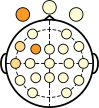
\includegraphics[width=0.15\textwidth]{./img_art_dfa/cabeza_new_MFGR_30.pdf} \\
VCR & MJH & JAE & GHA & MFGR \\
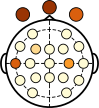
\includegraphics[width=0.15\textwidth]{./img_art_dfa/cabeza_new_CLO_30.pdf} &
\includegraphics[width=0.15\textwidth]{./img_art_dfa/cabeza_new_RLO_30.pdf} &
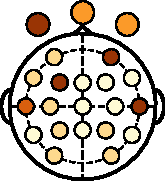
\includegraphics[width=0.15\textwidth]{./img_art_dfa/cabeza_new_RRU_30.pdf} &
\includegraphics[width=0.15\textwidth]{./img_art_dfa/cabeza_new_JGZ_30.pdf} &
\includegraphics[width=0.15\textwidth]{./img_art_dfa/cabeza_new_AEFP_30.pdf} \\
CLO & RLO & RRU & JGZ & AEFP
\end{tabular}
%\caption{En azul las zonas donde se encontraron diferencias significativas}
\end{figure}
\end{frame}

%%%%%%%%%%%%%%%%%%%%%%%%%%%%%%%%%%%%%%%%%%%%%%%%%
%%%%%%%%%%%%%%%%%%%%%%%%%%%%%%%%%%%%%%%%%%%%%%%%%

\begin{frame}\frametitle{MOR vs NMOR, grupal}
\begin{figure}
\centering
\includegraphics[width=0.8\linewidth]
{./img_art_dfa/Comparacion_gpos_CTL_PDC_v3.pdf} 
%\caption{ Promedio $\pm$ 1 desviaci\'on est\'andar. MOR: verde, NMOR: negro.}
\end{figure}
\end{frame}

\begin{frame}\frametitle{Gpo. Control vs Gpo. PDC}
\begin{figure}
\centering
\includegraphics[width=0.8\linewidth]
{./img_art_dfa/Comparacion_gpos_MOR_NMOR_v3.pdf} 
%\caption{ Promedio $\pm$ 1 desviaci\'on est\'andar. Control: azul, PDC: rojo.}
\end{figure}
\end{frame}

\subsection{Patrones visuales}

\begin{frame}\frametitle{Patrones visuales}
\begin{figure}
\includegraphics[width=0.95\textwidth]
{./img_art_dfa/zoom_noVCR_v2.png}
%\caption{Disposici\'on gr\'afica para los resultados de la prueba PSR. En verde el sue\~no MOR.}
\end{figure}
\end{frame}

\begin{frame}\frametitle{Patrones visuales: sueño MOR}
\begin{figure}
\includegraphics[width=0.95\textwidth]
{./img_art_dfa/zoom_siVCR_v2.png}
%\caption{Disposici\'on gr\'afica para los resultados de la prueba PSR. En verde el sue\~no MOR.}
\end{figure}
\end{frame}

\begin{frame}\frametitle{Los patrones son consistentes}
\begin{figure}
\begin{tabular}{c}
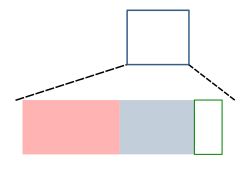
\includegraphics[width=0.3\textwidth]
{./img_ejemplos/zoom_VCR.pdf}
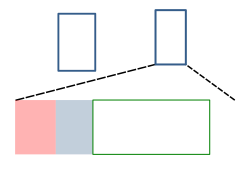
\includegraphics[width=0.3\textwidth]
{./img_ejemplos/zoom_MJH.pdf}
\includegraphics[width=0.3\textwidth]
{./img_ejemplos/zoom_JAE.pdf}
\\
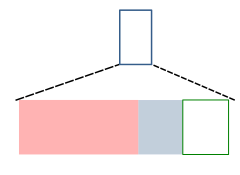
\includegraphics[width=0.3\textwidth]
{./img_ejemplos/zoom_GHA.pdf}
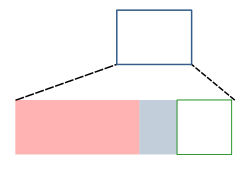
\includegraphics[width=0.3\textwidth]
{./img_ejemplos/zoom_MFGR.pdf}
\end{tabular}
%\caption{Patrones visuales que, se propone, est\'a asociado con la aparici\'on del sue\~no MOR}
\end{figure}
\end{frame}


\begin{frame}\frametitle{Estacionariedad y espectro de potencias}
\begin{figure}
\centering
\includegraphics[width=0.55\linewidth]
{./img_art_dfa/VCNNS1_espectral_total.png}
\end{figure}
\end{frame}


\begin{frame}\frametitle{Diferentes tamaños de ventana}
\begin{figure}
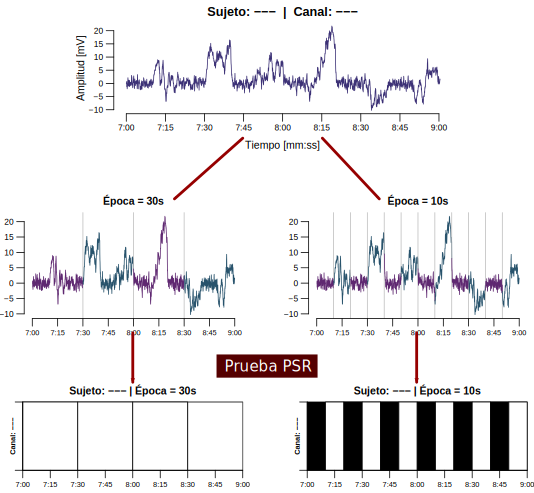
\includegraphics[width=0.7\textwidth]
{./img_diagramas/epocas_diferentes_v2.pdf}
%\caption{Disposici\'on gr\'afica para los resultados de la prueba PSR. En verde el sue\~no MOR.}
\end{figure}
\end{frame}

%%%%%%%%%%%%%%%%%%%%%%%%%%%%%%%%%%%%%%%%%%%%%%%%%
%%%%%%%%%%%%%%%%%%%%%%%%%%%%%%%%%%%%%%%%%%%%%%%%%

%\subsection{Discusi\'on}

\begin{frame}\frametitle{¿Ventanas muy grandes?}
\begin{figure}
\centering
\includegraphics[width=0.9\linewidth]
{./img_art_dfa/zoom_emergencia_VCR_120.png} 
\end{figure}
\end{frame}

\begin{frame}\frametitle{Ventanas de tamaño estándar}
\begin{figure}
\centering
\includegraphics[width=0.9\linewidth]
{./img_art_dfa/zoom_emergencia_VCR_30.png} 
\end{figure}
\end{frame}

\begin{frame}\frametitle{¿Ventanas muy chicas?}
\begin{figure}
\centering
\includegraphics[width=0.9\linewidth]
{./img_art_dfa/zoom_emergencia_VCR_7_5.png} 
\end{figure}
\end{frame}

\begin{frame}\frametitle{Escalamiento y homogeneidad}
\begin{figure}
\centering
\includegraphics[width=0.55\linewidth]
{./img_art_dfa/VCNNS1_comp_est_.png}
\end{figure}
\end{frame}

\begin{frame}\frametitle{¡Series de tiempo cortas y no-estacionarias!}
\begin{figure}
\centering
\includegraphics[width=.55\linewidth]{./img_resultados/cabeza_VCR.pdf}
%\caption{Cambio en el porcentaje de épocas estacionarias conforme el tamaño de ventana}
%\label{cabeza_repoio}
\end{figure}
\end{frame}

%%%%%%%%%%%%%%%%%%%%%%%%%%%%%%%%%%%%%%%%%%%%%%%%%
%%%%%%%%%%%%%%%%%%%%%%%%%%%%%%%%%%%%%%%%%%%%%%%%%

%\begin{frame}\frametitle{Sobre el tama\~no de la \'epoca}
%{\small Estacionariedad local\footcite{Cohen77}}
%\begin{figure}
%\centering
%\begin{tabular}{c}
%\includegraphics[width=0.4\linewidth]
%{./img_ejemplos/VCNNS1_est_30.png} \\
%\begin{tabular}{cc}
%\includegraphics[width=0.4\linewidth]
%{./img_ejemplos/VCNNS1_est_60.png} 
%&
%\includegraphics[width=0.4\linewidth]
%{./img_ejemplos/VCNNS1_est_10.png} 
%\end{tabular}
%\end{tabular}
%\end{figure}
%\end{frame}

%%%%%%%%%%%%%%%%%%%%%%%%%%%%%%%%%%%%%%%%%%%%%%%%%%%%%%%%%%%%%%%%%%%%%%%%%%%%%%%%%%%%%%%%%%%%%%%%%%%
%%%%%%%%%%%%%%%%%%%%%%%%%%%%%%%%%%%%%%%%%%%%%%%%%%%%%%%%%%%%%%%%%%%%%%%%%%%%%%%%%%%%%%%%%%%%%%%%%%%

\subsection{Conclusiones}

\begin{frame}\frametitle{Conclusiones}
\begin{itemize}
\item Presencia proporcional de estacionariedad d\'ebil, significativamente diferente en MOR vs 
NMOR en grupo Control

%\item An\'alisis para un AM con par\'alisis facial, detect\'o este padecimiento

%\item Consistente con trabajos anteriores %\cite{Valeria}

\item Patrones visuales, predicen parcialmente sue\~no MOR

\item Registros de PSG en AM, localmente estacionarias
\end{itemize}
\end{frame}

%%%%%%%%%%%%%%%%%%%%%%%%%%%%%%%%%%%%%%%%%%%%%%%%%%%%%%%%%%%%%%%%%%%%%%%%%%%%%%%%%%%%%%%%%%%%%%%%%%%
%%%%%%%%%%%%%%%%%%%%%%%%%%%%%%%%%%%%%%%%%%%%%%%%%%%%%%%%%%%%%%%%%%%%%%%%%%%%%%%%%%%%%%%%%%%%%%%%%%%

\section*{Gracias por su atención}

\begin{frame}\frametitle{Gracias por su atención}
\begin{figure}%[H]
\centering
\begin{tabular}{lc}
El cerebro es, quizá,\\
el único órgano del\\
cuerpo humano capaz \\
de estudiarse \\
as sí mismo\\
&
\includegraphics[width = 0.35\textwidth]{frase.png} 
\end{tabular}
\end{figure}
\end{frame}

%%%%%%%%%%%%%%%%%%%%%%%%%%%%%%%%%%%%%%%%%%%%%%%%%

\end{document}

%%%%%%%%%%%%%%%%%%%%%%%%%%%%%%%%%%%%%%%%%%%%%%%%%%%%%%%%%%%%%%%%%%%%%%%%%%%%%%%%%%%%%%%%%%%%%%%%%%%